\documentclass[12pt]{article}

\usepackage{amsmath}
\usepackage{amssymb}
\usepackage{anyfontsize}
\usepackage[toc,page]{appendix}
\usepackage{array}
\usepackage{booktabs}
\usepackage{caption}
\usepackage{cellspace}
\usepackage{color}
\usepackage{enumerate}
\usepackage{enumitem}
\usepackage{float}
\usepackage{geometry}
\usepackage{graphicx}
\usepackage{newtxtext,newtxmath}
\usepackage{listings}
\usepackage{physics} 
\usepackage{subfigure}
\usepackage{tabularx}

\geometry{
    a4paper,
    total = {170mm, 257mm},
    left = 20mm,
    top = 20mm,
    }

\definecolor{dkgreen}{rgb}{0,0.6,0}
\definecolor{gray}{rgb}{0.5,0.5,0.5}
\definecolor{mauve}{rgb}{0.58,0,0.82}
\lstset{frame = tb,
        language = Python,
        aboveskip = 3mm,
        belowskip = 3mm,
        showstringspaces = False,
        columns = flexible,
        basicstyle = {\small\ttfamily},
        numbers = left,
        numberstyle = \tiny\color{gray},
        keywordstyle = \color{blue},
        commentstyle = \color{dkgreen},
        stringstyle = \color{mauve},
        breaklines = true,
        breakatwhitespace = true,
        tabsize=4}

\renewcommand\lstlistingname{Algorithm}
\captionsetup[lstlisting]{singlelinecheck=false, margin=12pt, labelsep=default, labelfont=default}
%We can also use: labelsep=period or labelsep=spacce, labelfont=default or labelfont=bf


%%%%%%%%%%%%%%%%%%%%%%%%%%%%%%%%%%% Again, Don't change anything Above %%%%%%%%%%%%%%%%%%%%%%%%%%%%%%%%%%%


\begin{document}

\title{\textbf{{\normalsize Computational Physics Lab}\\
                Homework 4}}
\author{108000204\\
        Yuan-Yen Peng\\
        \textit{Dept. of Physics, NTHU}\\
        \textit{Hsinchu, Taiwan}}
\date{\today}
\maketitle

\section{Writing Assignments}
    \subsection{Finite difference method for solving 2D Poisson equation}
    The $3 \times 3$ grids with grid space $h$ and the source term $\rho(x,y)$ can be described as:
    \[
        u_{xx} + u_{yy} = \rho(x,y)
    \]
    where the subscripts mean second partial derivatives of the u with $x$ and $y$, respectively. Besides, we annotate $(x,y)$ with $(i,j)$ where $i$ and $j$ are from $0 \sim (3+1)$ (including boundaries, which are $(i,j) = (i,0),\ (i,4),\ (0,j),\text{and}\ (4,j)$), and implement the Euler method for derivative; then we can get:
    \begin{align*}
        &\frac{\partial}{\partial x}\Big( \frac{u_{i,j} - u_{i-1,j}}{h} \Big) + \frac{\partial}{\partial y}\Big( \frac{u_{i,j} - u_{i,j-1}}{h} \Big) = \rho(x,y) \\
        \Rightarrow &\frac{1}{h} \Big( \frac{u_{i+1,j} - u_{i,j}}{h} - \frac{u_{i,j} - u_{i-1,j}}{h} \Big) + \frac{1}{h} \Big( \frac{u_{i,j+1} - u_{i,j}}{h} - \frac{u_{i,j} - u_{i,j-1}}{h} \Big) = \rho(x,y) \\
        \Rightarrow &\big( u_{i+1,j} - 2u_{i,j} + u_{i-1,j} \big) + \big( u_{i,j+1} - 2u_{i,j} + u_{i,j-1} \big) = \rho(x,y) h^{2} \\
        \Rightarrow&\ 4_{i,j} - u_{i-1,j} - u_{i+1,j} - u_{i,j-1} - u_{i,j+1} = \rho(x,y) h^{2} \tag{I}\label{A}
    \end{align*}
    In the wake of knowing the general form of the solution, we apply the boundary conditions; here boundaries are all zeros (i.e., $u_{0,j},\ u_{i,0},\ u_{4,j},\ \text{and}\ u_{i,4} = 0$). Exploiting all $i$ and $j$, we can get LHS of eq.(\ref{A}) in the matrix form $\mathbf{A}$ and RHS in the vector form $\mathbf{b}$ with source term $g_{ij}$ which represents the splitting of the source function $\rho(x,y)$:
    \[
        \mathbf{A} = 
        \begin{bmatrix}
            \begin{bmatrix}
                4  & -1 & 0 \\
                -1 & 4  & -1\\
                0  & -1 & 4 \\
            \end{bmatrix}
            &
            \begin{bmatrix}
                -1 & 0  & 0 \\
                0  & -1 & 0 \\
                0  & 0  & -1\\
            \end{bmatrix}
            &
            \begin{bmatrix}
                0 & 0 & 0 \\
                0 & 0 & 0 \\
                0 & 0 & 0\\
            \end{bmatrix}
            \\
            \\
            \begin{bmatrix}
                -1 & 0  & 0 \\
                0  & -1 & 0 \\
                0  & 0  & -1\\
            \end{bmatrix}
            &
            \begin{bmatrix}
                4  & -1 & 0 \\
                -1 & 4  & -1\\
                0  & -1 & 4 \\
            \end{bmatrix}
            &
            \begin{bmatrix}
                -1 & 0  & 0 \\
                0  & -1 & 0 \\
                0  & 0  & -1\\
            \end{bmatrix}
            \\
            \\
            \begin{bmatrix}
                0 & 0 & 0 \\
                0 & 0 & 0 \\
                0 & 0 & 0\\
            \end{bmatrix}
            &
            \begin{bmatrix}
                -1 & 0  & 0 \\
                0  & -1 & 0 \\
                0  & 0  & -1\\
            \end{bmatrix}
            &
            \begin{bmatrix}
                4  & -1 & 0 \\
                -1 & 4  & -1\\
                0  & -1 & 4 \\
            \end{bmatrix}
        \end{bmatrix}
    \]
    and 
    \[
        \mathbf{b} = -h^{2}
        \begin{bmatrix}
            g_{11}\\
            g_{12}\\
            g_{13}\\
            ---\\
            g_{21}\\
            g_{22}\\
            g_{23}\\
            ---\\
            g_{31}\\
            g_{32}\\
            g_{33}\\
        \end{bmatrix}
    \]

    \section{Programming Assignments}
    \subsection{$\rho_{22} = 1$ and else are zeros}
    Homework's figure in the last problem is $4 \times 4$, but the question asks the $3 \times 3$ matrix. Thus, I generate the two results in Figure\ref{q1}, the left one uses the definition of the left bottom corner, and the other (right) implements the center of the grid as a benchmark.

    \begin{figure}[H]
        \centering 
        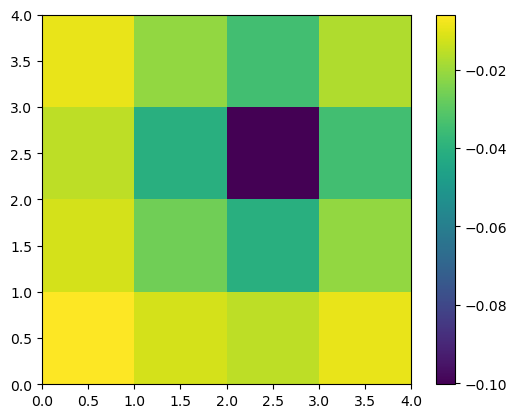
\includegraphics[width = 0.45\textwidth]{./fig/1.1.png}
        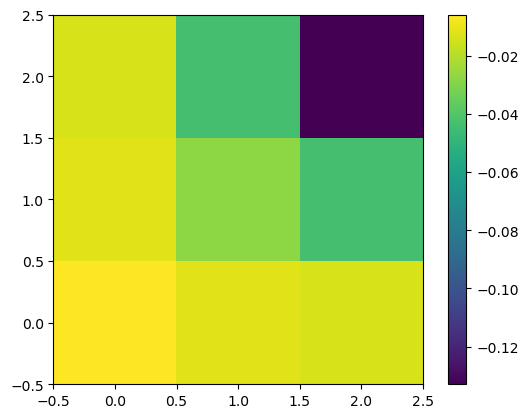
\includegraphics[width = 0.45\textwidth]{./fig/1.2.png} 
        \caption{These figures are the solution of the potential $u$. The left is the $4 \times 4$ grid; the right is the $3 \times 3$ grid. Both of them are with the source $\rho_{22} = 1$ and the others are zeros.}\label{q1}
    \end{figure}

    \subsection{2D Poisson's equation with a given source with periodic boundary}\label{eq}
    In this subsection (also the below's subsections), we exploit the finite difference method with the sparse matrix to solve the equation:
    \[
        \rho(x,y) = e^{-{5 \over 4} r^{2}_{1}} + {3 \over 2} \times e^{-r^{2}_{2}}
    \]
    with the domain $\mathscr{D}\big\{ [-5 < x < 5] \times [-5 < y < 5] \big\}$ in the $128 \times 128$ grid.

    \begin{figure}[H]
        \centering
        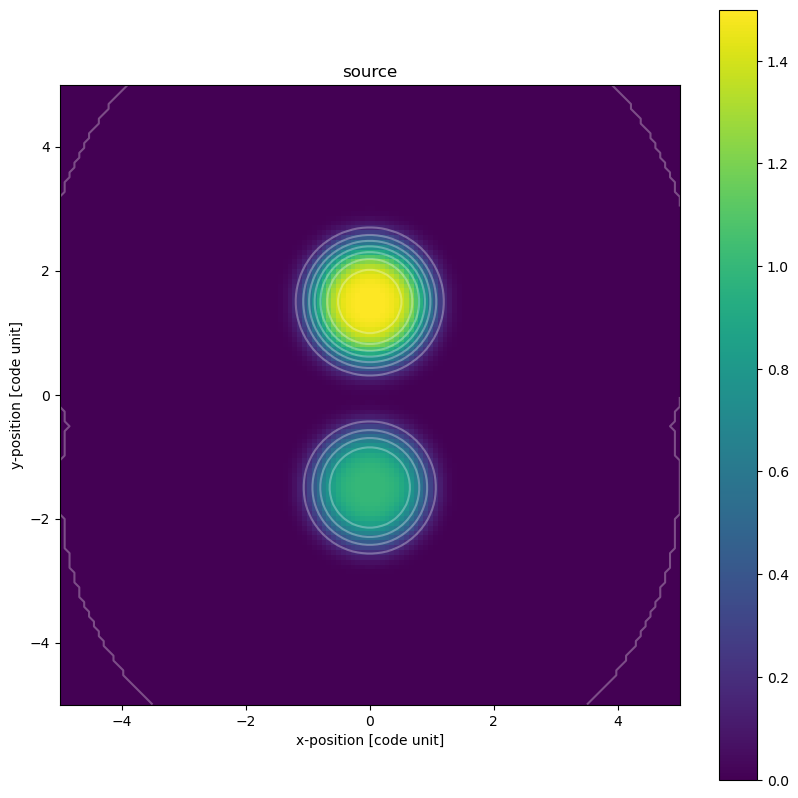
\includegraphics[width = 0.45\textwidth]{./fig/2.1.png}
        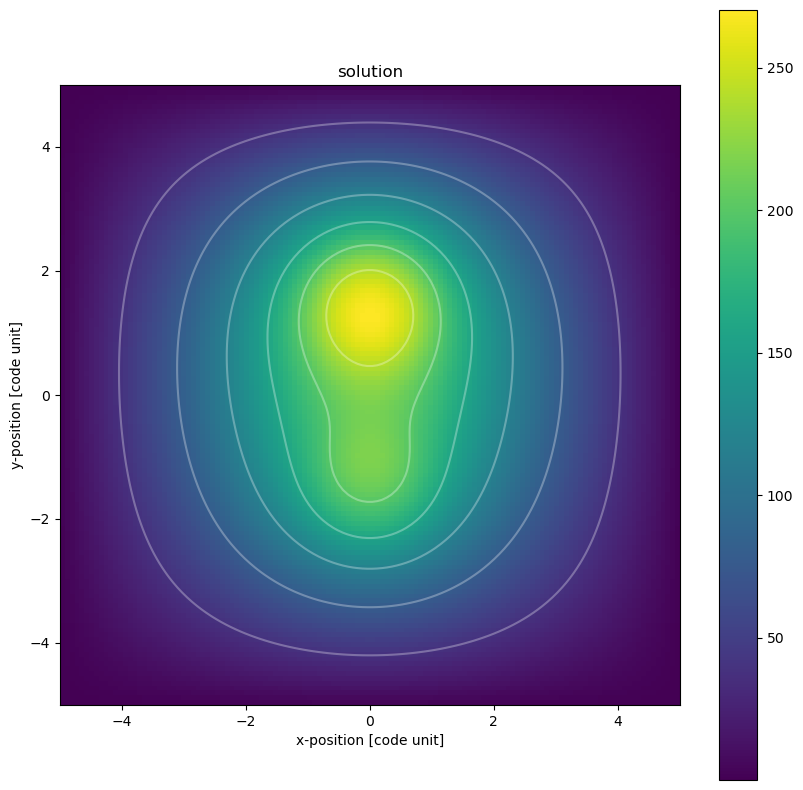
\includegraphics[width = 0.45\textwidth]{./fig/2.2.png}
        \caption{The left is the source function with the scheme with periodic boundary; the right is the solution of the corresponding potential for this Poisson's equation also with the periodic boundary exploiting the sparse matrix method. Moreover, this ``periodic boundary'' will be updated in each run during finite difference algorithm execution.}
    \end{figure}

    \subsection{Error convergence comparison between different algorithms}
    We utilize three different methods learned in the lecture to investigate the error convergence of this Poisson's equation. The first method we used is the Jacobi method and the second is the Gauss-Seidel method, and the last method is the successive over-relaxation method with $w = 1.2,\ 1,5,\text{and}\ 2.0$. However, in SOR (successive over-relaxation method), it might be ``diverge'', so we plot two schemes to research the convergence rate, one is all converge and the other is one of them diverge, please see in Figure\ref{q3}.

    \begin{figure}[H]
        \centering
        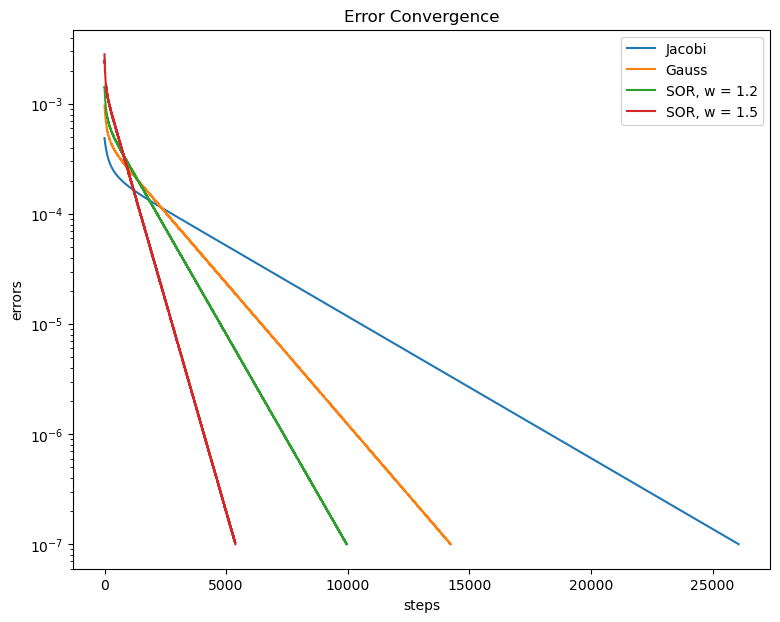
\includegraphics[width = 0.45\textwidth]{./fig/3.1.png}
        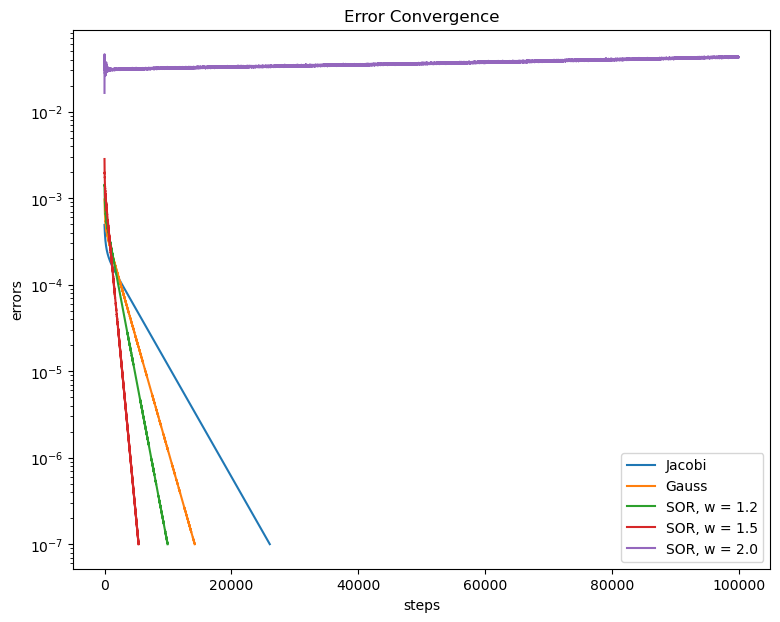
\includegraphics[width = 0.45\textwidth]{./fig/3.2.png}
        \caption{These two figures have the log-scale y-axis; normal scale x-axis so as to show errors as functions of iterations. Here, we use the error defined by $\sqrt{\sum (u[i,j]-u_{old}[i,j])^{2}} / (\text{number of cells})$.\\
        The left is all the methods are converged; the right scheme is the one diverge situation ($w = 2.0$, purple line).}\label{q3}
    \end{figure}

    It is manifestly that the Jacobi method is the slowest one and then is the Gauss-Seidel method, and the fastest is the SOR method. In this scenario, although SOR is the fastest when $w = 1.5$, it will diverge with $w = 2.0$ (Figure\ref{q3}-right)! The fastest (SOR with $w = 1.5$) is approximately 4.5 times faster than the slowest (Jacobi) as the error tolerance is $\sim 10^{-6}$.

    \subsection{Resolution vs time with different methodologies}
    In this subsection, we will discuss different grid sizes; that is, different resolutions ($32 \times 32$, $64 \times 64$, and $128 \times 128$) with the time. Additionally, we exploit the methods of the sparse matrix, Jacobi, Gauss-Seidel, and SOR with $w = 1.2,\ 1.5$ as well. Setting tolerance $\epsilon = 10^{-7}$, the resolutions vs time show in Figure\ref{q4}.

    \begin{figure}[H]
        \centering
        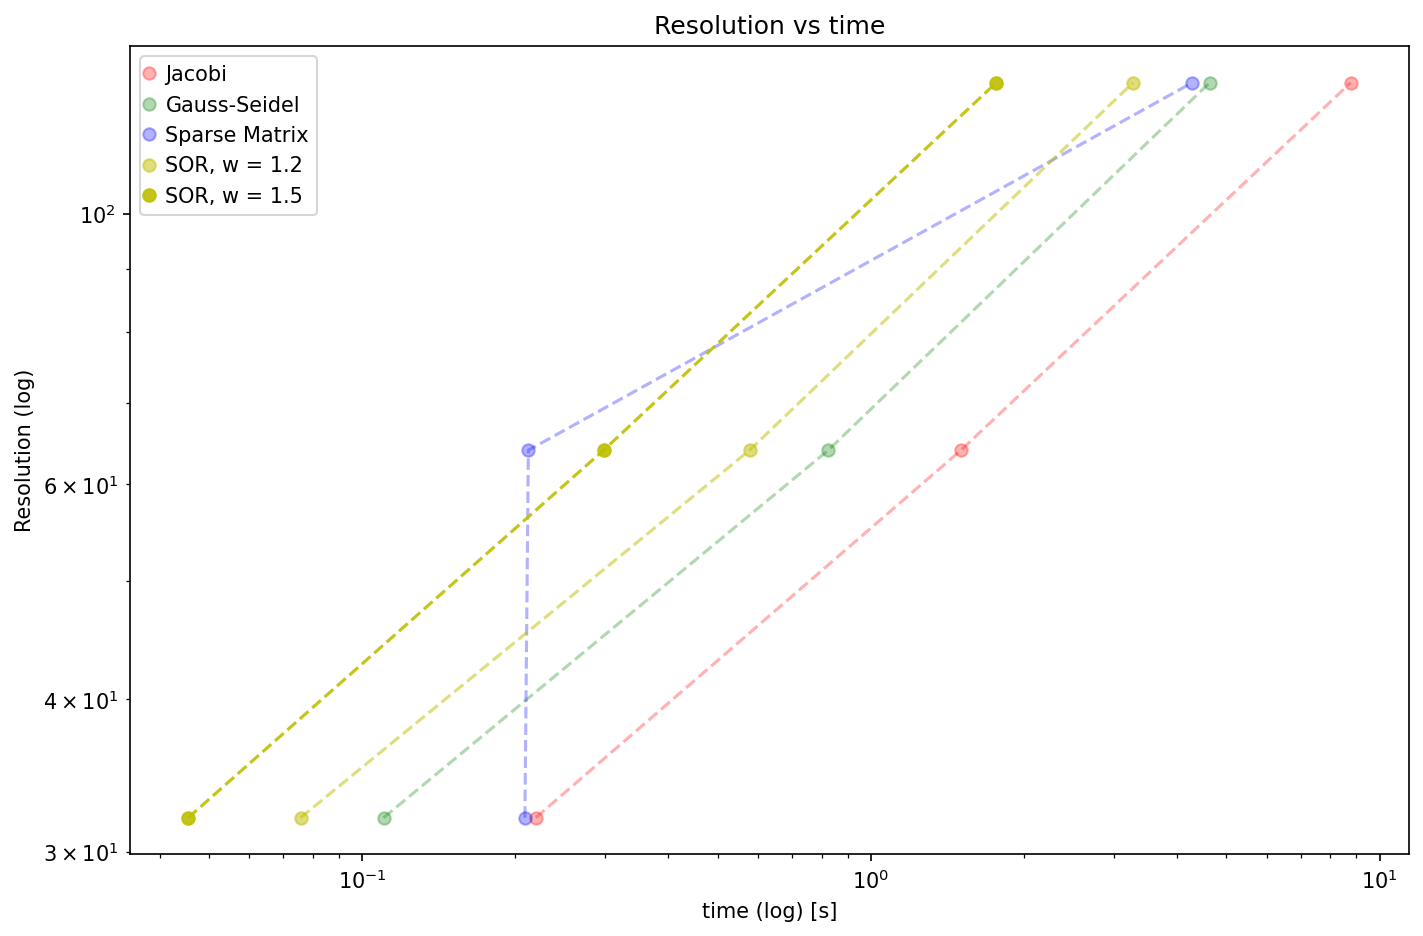
\includegraphics[width = 0.9\textwidth]{./fig/4.png}
        \caption{This figure shows different algorithms to solve Poisson's equation in (subsection \ref{eq}). The tendency of these methods, excluding sparse matrix, require more time to iterate to the tolerance ($\epsilon = 10^{-7}$). The outcomes are the same consequent analysis in the aforementioned subsections; i.e., Jacobi is the slowest, Gauss-Seidel is the middle and the SOR is the fastest (besides, $w = 1.5$ is more efficient than $w = 1.3$). On the other hand, the behavior of the sparse matrix method does not act the same as others. It takes the least time among others when the resolution is $64 \times 64$. Likewise, in low resolution ($32 \times 32$), the sparse matrix method is only faster than Jacobi, but in the largest resolution ($128 \times 128$), it drills faster than Jacobi and also the Gauss-Seidel. Here, we can briefly sum up, if the size (resolution) is in ``some proper range'', such as $64 \times 64$, we can adopt \texttt{SciPy}'s sparse solver! It is more well organized than others.}\label{q4}
    \end{figure}

\section{Codes}
    All the codes are transferred from JupyterLab or python codes; hence, if you want to re-run them, please see the source code in the attached files or my GitHub repository:

    {\centerline{\ttfamily <https://github.com/gary20000915/Comphyslab-HW4.git>}}

    \subsection{\texttt{solvers.py}}
        \begin{lstlisting}[language={Python}]
            import numpy as np
            from numba import njit, prange
            
            from .mesh import Mesh2D
            
            """
            Solver to solve for Laplace/Poisson's equation
            
            """
            
            @njit(parallel=True)
            def generate_g(g, buff_size, nx, ny, x, y):
                for i in prange(nx+2*buff_size):
                    for j in prange(ny+2*buff_size):
                        r1 = np.square(x[i] + 1.5) + np.square(y[j])
                        r2 = np.square(x[i] - 1.5) + np.square(y[j])
                        g[i, j] = np.exp(-5 * 0.25 * np.square(r1)) + 3 * 0.5 * np.exp(-np.square(r2))
            
                return g
            
            def set_boundary(g, x, y, nx, ny, buff_size, mesh: Mesh2D):
                generate_g(g, buff_size, nx, ny, x, y)
                UL = g[-1,:]
                LR = g[:,-1]
                boundary = np.array([[UL],[LR],[UL],[LR]])
                mesh[0, :] = boundary[0]
                mesh[ny+buff_size, :] = boundary[1]
                mesh[:, 0]  = boundary[2]
                mesh[:, nx+buff_size] = boundary[3]
            
            
            @njit(parallel = True)
            def j_kernel(u, u_temp, x, y, nx, ny, g, buff_size):
                for i in prange(1, nx + 2*buff_size - 1, 1):
                    for j in prange(1, ny + 2*buff_size - 1, 1):
                        r1 = np.square(x[i] + 1.5) + np.square(y[j])
                        r2 = np.square(x[i] - 1.5) + np.square(y[j])
                        g[i, j] = np.exp(-5 * 0.25 * np.square(r1)) + 3 * 0.5 * np.exp(-np.square(r2))
                        u[i, j] = 0.25 * (u_temp[i+1, j] + u_temp[i, j+1] + u_temp[i-1, j] + u_temp[i, j-1] + g[i, j])
                return u
                
            @njit(parallel = True)
            def gs_kernel(u, x, y, nx, ny, g, buff_size):
                for i in prange(1, nx + 2*buff_size - 1, 1):
                    for j in prange(1, ny + 2*buff_size - 1, 1):
                        r1 = np.square(x[i] + 1.5) + np.square(y[j])
                        r2 = np.square(x[i] - 1.5) + np.square(y[j])
                        g[i, j] = np.exp(-5 * 0.25 * np.square(r1)) + 3 * 0.5 * np.exp(-np.square(r2))
                        u[i, j] = 0.25 * (u[i+1, j] + u[i, j+1] + u[i-1, j] + u[i, j-1] + g[i, j])
                return u
            
            @njit(parallel = True)
            def SOR_kernel(u, u_temp, x, y, nx, ny, g, buff_size, w):
                for i in prange(1, int(nx + 2*buff_size - 1), 1):
                    for j in prange(1, int(ny + 2*buff_size - 1), 1):
                        r1 = np.square(x[i] + 1.5) + np.square(y[j])
                        r2 = np.square(x[i] - 1.5) + np.square(y[j])
                        g[i, j] = np.exp(-5 * 0.25 * np.square(r1)) + 3 * 0.5 * np.exp(-np.square(r2))
                        u[i, j] = 0.25 * (u[i+1, j] + u[i, j+1] + u[i-1, j] + u[i, j-1] + g[i, j])
                        u[i, j] = (1-w) * u_temp[i,j] + w * u[i, j]
                return u
            
            def solve(name, tor, mesh: Mesh2D, **kwargs):
                u         = mesh.get_mesh()
                x         = mesh.get_x()
                y         = mesh.get_y()
                nx        = mesh.get_nx()
                ny        = mesh.get_ny()
                g         = mesh.get_xx()
                buff_size = mesh.get_buff_size()
                
                err     = 10
                err_arr = np.array([])
                n       = 0
                
                while err > tor:
                    u_temp = np.copy(u)
                    set_boundary(g, x, y, nx, ny, buff_size, u)
                    
                    if name == "Jacobi":
                        u = j_kernel(u, u_temp, x, y, nx, ny, g, buff_size)
                    elif name == "Gauss":
                        u = gs_kernel(u, x, y, nx, ny, g, buff_size)
                    elif name == "SOR":
                        u = SOR_kernel(u, u_temp, x, y, nx, ny, g, buff_size, kwargs['w'])
                    else:
                        print("Error: unknown kernel!")
                        break
            
                    err = np.sqrt(np.sum(np.square(u - u_temp))) / (nx * ny)
                    err_arr = np.append(err_arr, err)
                    n += 1
                    # check
                    # if n % 100 == 0:
                    #     print(err, tor)
                        # print(u)
                        # plt.imshow(u.reshape(nx+2*buff_size, ny+2*buff_size), origin = 'lower', extent=[-1, 1, -1, 1])
                        # plt.colorbar()
                        # plt.contour(u, colors = 'white', extent=[-1, 1, -1, 1])
                    if n == 1e5:
                        break
                    
                return u.reshape(nx+2*buff_size, ny+2*buff_size), err_arr, n
            
            
            
            if __name__=='__main__':
            
                nx, ny = 4, 4
                buff_size=1
                tor = 1e-10
                # boundary = np.zeros((4, nx + 2*buff_size))
                # boundary[0] =np.ones(nx + 2*buff_size)
                mesh = Mesh2D(nx = nx, ny = ny, buff_size=buff_size)
            
                u = solve("Jacobi", tor, mesh)[1]
                print(u)
                print("TEST")
        \end{lstlisting}

    \subsection{\texttt{mesh.py}}
        \begin{lstlisting}[language={Python}]
            """
            This file define classes for generating 2D meshes.
            
            """
            import numpy as np
            from numba import jit, int32, float64
            from numba.experimental import jitclass
            
            class Mesh2D:
                def __init__(self, nx:int = 10, ny:int = 10, buff_size = 1, xmin = 0, xmax = 1, ymin = 0, ymax = 1):
                    self._nx = nx
                    self._ny = ny
                    self._nbuff = buff_size
                    self._xmin = xmin
                    self._xmax = xmax
                    self._ymin = ymin
                    self._ymax = ymax   
                    
                    self._setup()
                    
                    return
            
                def _setup(self):
                    self._dx = (self._xmax - self._xmin) / (self._nx + 1)
                    self._dy = (self._ymax - self._ymin) / (self._ny + 1)
                    
                    self._istart = self._nbuff
                    self._istartGC = 0
                    self._iend = self._nbuff + self._nx - 1
                    self._iendGC = 2 * self._nbuff + self._nx - 1
                    self._nxGC = 2 * self._nbuff + self._nx
                    
                    self._jstart = self._nbuff
                    self._jstartGC = 0
                    self._jend = self._nbuff + self._ny - 1
                    self._jendGC = 2 * self._nbuff + self._ny - 1
                    self._nyGC = 2 * self._nbuff + self._ny
                    
                    x = np.linspace(self._xmin, self._xmax, self._nxGC)
                    y = np.linspace(self._ymin, self._ymax, self._nyGC)
                    xx, yy = np.meshgrid(x, y, indexing='ij')
                    self._mesh = xx * 0
                    self._xx = xx
                    self._yy = yy
                    self._x = x
                    self._y = y
                    
                    return
                    
                def get_nx(self):
                    return int(self._nx)
                def set_nx(self, nx):
                    self._nx = nx
                    self._setup()
                    return
            
                def get_ny(self):
                    return int(self._ny)
                def set_ny(self, ny):
                    self._ny = ny
                    self._setup()
                    return
            
                def get_buff_size(self):
                    return int(self._nbuff)
                def set_buff_size(self, buff_size):
                    self._nbuff = buff_size
                    self._setup()
                    return
            
                def get_xmin(self):
                    return self._xmin
                def set_xmin(self, xmin):
                    self._xmin = xmin
                    self._setup()
                    return 
            
                def get_xmax(self):
                    return self._xmax
                def set_xmax(self, xmax):
                    self._xmax = xmax
                    self._setup()
                    return 
            
                def get_ymin(self):
                    return self._ymin
                def set_ymin(self, ymin):
                    self._ymin = ymin
                    self._setup()
                    return
            
                def get_ymax(self):
                    return self._ymax
                def set_ymax(self, ymax):
                    self._ymax = ymax
                    self._setup()
                    return
            
                def get_istart(self):
                    return self._istart
                def set_istart(self, istart):
                    self._istart = istart
                    self._setup()
                    return
            
                def get_istartGC(self):
                    return self._istartGC
                def set_istartGC(self, istartGC):
                    self._istartGC = istartGC
                    self._setup()
                    return
            
                def get_iend(self):
                    return self._iend
                def set_iend(self, iend):
                    self._iend = iend
                    self._setup()
                    return
                
                def get_iendGC(self):
                    return self._iendGC
                def set_iendGC(self, iendGC):
                    self._iendGC = iendGC
                    self._setup()
                    return
            
                def get_jstart(self):
                    return self._jstart
                def set_jstart(self, jstart):
                    self._jstart = jstart
                    self._setup()
                    return
            
                def get_jstartGC(self):
                    return self._jstartGC
                def set_jstartGC(self, jstartGC):
                    self._jstartGC = jstartGC
                    self._setup()
                    return
            
                def get_jend(self):
                    return self._jend
                def set_jend(self, jend):
                    self._jend = jend
                    self._setup()
                    return
                
                def get_jendGC(self):
                    return self._jendGC
                def set_jendGC(self, jendGC):
                    self._jendGC = jendGC
                    self._setup()
                    return
            
                def get_mesh(self):
                    return self._mesh
                def set_mesh(self, mesh):
                    self._mesh = mesh
                    if (mesh.size != self._mesh.size): 
                        print("error! size conflict!")
                    return
                
                def get_xx(self):
                    return self._xx
                def set_xx(self, xx):
                    self._xx = xx
                    self._setup()
                    return
            
                def get_yy(self):
                    return self._yy
                def set_yy(self, yy):
                    self._yy = yy
                    self._setup()
                    return
                
                def get_x(self):
                    return self._x
                def set_x(self, x):
                    self._x = x
                    self._setup()
                    return
            
                def get_y(self):
                    return self._y
                def set_y(self, y):
                    self._y = y
                    self._setup()
                    return
            
                def get_nx(self):
                    return self._nx
                def set_nx(self, nx):
                    self._nx = nx
                    self._setup()
                    return
                
                def get_ny(self):
                    return self._ny
                def set_ny(self, ny):
                    self._ny = ny
                    self._setup()
                    return
            
            
            if __name__=='__main__':
                mesh = Mesh2D(nx = 3, ny = 3, buff_size=1)
                # mesh.set_nx(32)
                # mesh.set_ny(32)
                
                u = mesh.get_mesh()
                nx = mesh.get_nx()
                ny = mesh.get_ny()
                buff = mesh.get_buff_size()
            
                print(u)
                print(f"Testing ... nx={nx}, ny={ny}, buff ={buff}")
                print('Done')
        \end{lstlisting}

    \subsection{\texttt{1\_finite\_difference.ipynb}}
        \begin{lstlisting}[language={Python}]
            # %% [markdown]
            # ### 1. Finite Difference method for solving discrete Laplace Equation
            
            # %%
            %reset -f
            
            import numpy as np
            import matplotlib.pyplot as plt
            from scipy import linalg
            from scipy.sparse import csc_matrix
            from scipy.sparse import dia_array
            from scipy.sparse import dia_matrix
            import scipy.sparse.linalg as splinalg
            from numba import njit, prange
            
            # %%
            N = 4
            min, max = -1, 1
            dx = (max - min) / N
            
            # %%
            def generate_D(n):
                ex = np.ones(n)
                data = np.array([-1 * ex, 4 * ex, -1 * ex])
                offsets = np.array([-1, 0, 1])
                
                return dia_matrix((data, offsets), shape=(n, n)).toarray()
            
            # %%
            @njit(parallel = True)
            def kernel(N, A, D, I):
                for i in prange(N):
                    for j in prange(N):
                        if i == j:
                            for ii in prange(N):
                                for jj in prange(N):
                                    A[ii+N*i, jj+N*j] = D[ii, jj]
                                    
                        if np.abs(i - j) == 1:
                            for ii in prange(N):
                                for jj in prange(N):
                                    A[ii+N*i, jj+N*j] = I[ii, jj]
                                    
                return A
            
            # %%
            def generate_A(N):
                A = np.zeros((N ** 2, N ** 2))
                D = generate_D(N)
                I = -np.identity(N)
                A = kernel(N, A, D, I)
                return A
            
            # %%
            def generate_b(N, dx):
                b = np.zeros(N ** 2).reshape(N, N)
                b[2, 2] = -1 * np.square(dx)
                plt.imshow(b, origin = 'lower')
                plt.colorbar()
                return b.reshape(N ** 2)
            
            # %%
            # solve
            def solve(N, dx):
                a = generate_A(N)
                a = csc_matrix(a) # transform to the fitting matrix
                b = generate_b(N, dx)
                x = splinalg.spsolve(a, b).reshape(N, N)
                return x
            
            # %%
            u = solve(N, dx)
            print(u)
            
            # %%
            plt.imshow(u, origin = 'lower', extent = [0,4,0,4])
            plt.colorbar()            
        \end{lstlisting}


    \subsection{\texttt{2\_finite\_difference.ipynb}}
        \begin{lstlisting}[language={Python}]
            # %% [markdown]
            # ### Finite Difference method for solving discrete Laplace Equation
            
            # %%
            %reset -f
            
            import numpy as np
            import matplotlib.pyplot as plt
            from matplotlib.pyplot import figure
            from scipy import linalg
            from scipy.sparse import csc_matrix
            from scipy.sparse import dia_array
            from scipy.sparse import dia_matrix
            import scipy.sparse.linalg as splinalg
            from numba import njit, prange
            
            # %%
            N = 128
            min, max = -5, 5
            dx = (max - min) / N
            
            x = np.linspace(-5, 5, N)
            y = np.linspace(-5, 5, N)
            g = np.zeros([N, N])
            
            # %%
            def generate_D(n):
                ex = np.ones(n)
                data = np.array([-1 * ex, 4 * ex, -1 * ex])
                offsets = np.array([-1, 0, 1])
                
                return dia_matrix((data, offsets), shape=(n, n)).toarray()
            
            # %%
            @njit
            def kernel(N, A, D, I):
                for i in prange(N):
                    for j in prange(N):
                        if i == j:
                            for ii in prange(N):
                                for jj in prange(N):
                                    A[ii+N*i, jj+N*j] = D[ii, jj]
                                    
                        if np.abs(i - j) == 1:
                            for ii in prange(N):
                                for jj in prange(N):
                                    A[ii+N*i, jj+N*j] = I[ii, jj]
                                    
                return A
            
            # %%
            def generate_A(N):
                A = np.zeros((N ** 2, N ** 2))
                D = generate_D(N)
                I = -np.identity(N)
                A = kernel(N, A, D, I)
                return A
            
            # %%
            @njit
            def generate_g(g, N, x, y):
                for i in prange(N):
                    for j in prange(N):
                        r1 = np.square(x[i] + 1.5) + np.square(y[j])
                        r2 = np.square(x[i] - 1.5) + np.square(y[j])
                        g[i, j] = np.exp(-5 * 0.25 * np.square(r1)) + 3 * 0.5 * np.exp(-np.square(r2))
            
                return g
            
            # %%
            ans = generate_g(g, N, x, y)
            
            figure(figsize=(10, 10), dpi=100)
            plt.imshow(ans, origin = 'lower', extent=[-5, 5, -5, 5])
            plt.colorbar()
            plt.contour(ans, colors = 'w', alpha = .3, extent=[-5, 5, -5, 5])
            plt.title('source')
            plt.xlabel('x-position [code unit]')
            plt.ylabel('y-position [code unit]')
            plt.show()
            plt.close()
            
            # %%
            def generate_b(N, g, dx):
                # boundaries
                # b = np.zeros(N ** 2)
                b = g.reshape(N, N)
                b[-1,:] = b[1,: ]
                b[:,-1] = b[:,-1]
                b = b.reshape(N ** 2)
                # source
                b += - g * np.square(dx)
                return b
            
            # %%
            # solve
            def solve(N, g, dx, x, y):
                g = generate_g(g, N, x, y).reshape(N ** 2)
                a = generate_A(N)
                a = csc_matrix(a) # transform to the fitting matrix
                b = generate_b(N, g, dx)
                x = splinalg.spsolve(a, b).reshape(N, N)
                return x
            
            # %%
            u = solve(N, g, dx, x, y)
            # %timeit solve(N, g, dx, x, y)
            
            # %% [markdown]
            # parallel: 6.31 s ± 29.3 ms per loop (mean ± std. dev. of 7 runs, 1 loop each)  
            # nopython: 6.08 s ± 136 ms per loop (mean ± std. dev. of 7 runs, 1 loop each)
            
            # %%
            figure(figsize=(10, 10), dpi=100)
            plt.imshow(u, origin = 'lower', extent=[-5, 5, -5, 5])
            plt.colorbar()
            plt.contour(u, colors = 'w', alpha = .3, extent=[-5, 5, -5, 5])
            plt.title('solution')
            plt.xlabel('x-position [code unit]')
            plt.ylabel('y-position [code unit]')
            plt.show()
            plt.close()            
        \end{lstlisting}

    \subsection{\texttt{3\_iteractive\_methods.ipynb}}
        \begin{lstlisting}[language={Python}]
            # %% [markdown]
            # # Laplace Equation & Possion Equations
            # 
            # In this Lab, we will learn how to numerically solve Laplace and Possion equations, which are common equations in electromagnestism and gravitational problems. 
            
            # %% [markdown]
            # There should be two files under `./poisson_solver`.\
            # 1. `mesh.py` handles the mesh grids we will used in this Lab.\
            # 2. `solvers.py` handles all corresponding iterative solvers for Laplace/Poisson Equation. 
            
            # %%
            %reset -f
            
            import numpy as np
            import numba as na
            import matplotlib.pyplot as plt
            from matplotlib.pyplot import figure
            import time as time
            from poisson_solver.mesh import Mesh2D
            from poisson_solver.solvers import *
            
            # %% [markdown]
            # ## Exercise 4: Jacobi method
            # 
            # 1. Test your Mesh2D class to see if you could generate the grids we need for this calculation
            # 2. Implement the Jacobi meothd in `./poisson_solver/solver.py`.
            # 3. Write a function called `updata_boundary()` to update the boundary conditions.\
            #    Where to put this `update_boundary()` function is up to you.\
            #    You could put it either inside the `Mesh2D` class, in `solvers.py`, or here.
            
            # %% [markdown]
            # ## Exercise 5: Gauss-Seidel Meothd.
            # 
            # 1. Implement the Gauss-Seidel meothd in your solver.
            # 2. Repeat exercise 4. for the Gauss-Seidel meothd.
            # 3. Compare the error convergence between Jacobi and Gauss-Seidel
            
            # %%
            def setup():
                tor       = 1e-7
                xmin, xmax = -5, 5
                ymin, ymax = -5, 5
                nx, ny    = 128, 128
                buff_size = 1
                
                mesh = Mesh2D(nx = nx, ny = ny, buff_size = buff_size)
                mesh.set_xmin(xmin)
                mesh.set_xmax(xmax)
                mesh.set_ymin(ymin)
                mesh.set_ymax(ymax)
            
                return tor, mesh
            
            # %%
            '''
            Jacobi
            '''
            ini = setup()
            t1 = time.time()
            # name == Gauss or Jacobi or SOR
            j_arr = solve("Jacobi", ini[0], ini[1])
            j_u   = j_arr[0]
            j_err = j_arr[1]
            j_n   = j_arr[2]
            j_N = np.linspace(0, int(j_n), int(j_n))
            t2 = time.time()
            
            '''
            Gauss-Seidel
            '''
            ini = setup()
            t3 = time.time()
            # name == Gauss or Jacobi or SOR
            g_arr = solve("Gauss", ini[0], ini[1])
            g_u   = g_arr[0]
            g_err = g_arr[1]
            g_n   = g_arr[2]
            g_N = np.linspace(0, int(g_n), int(g_n))
            t4 = time.time()
            
            '''
            SOR
            '''
            ini = setup()
            t5 = time.time()
            # name == Gauss or Jacobi or SOR
            w1, w2, w3 = 1.2, 1.5, 2.0
            
            s1_arr = solve("SOR", ini[0], ini[1], w = w1)
            s1_u   = s1_arr[0]
            s1_err = s1_arr[1]
            s1_n   = s1_arr[2]
            s1_N = np.linspace(0, int(s1_n), int(s1_n))
            # prune the margins
            s1_u = np.delete(s1_u, (0, -1), 0)
            s1_u = np.delete(s1_u, (0, -1), 1)
            
            ini = setup()
            s2_arr = solve("SOR", ini[0], ini[1], w = w2)
            s2_u   = s2_arr[0]
            s2_err = s2_arr[1]
            s2_n   = s2_arr[2]
            s2_N = np.linspace(0, int(s2_n), int(s2_n))
            # prune the margins
            s2_u = np.delete(s2_u, (0, -1), 0)
            s2_u = np.delete(s2_u, (0, -1), 1)
            
            ini = setup()
            s3_arr = solve("SOR", ini[0], ini[1], w = w3)
            s3_u   = s3_arr[0]
            s3_err = s3_arr[1]
            s3_n   = s3_arr[2]
            s3_N = np.linspace(0, int(s3_n), int(s3_n))
            # prune the margins
            s3_u = np.delete(s3_u, (0, -1), 0)
            s3_u = np.delete(s3_u, (0, -1), 1)
            t6 = time.time()
            
            print("Jocobi -> Time = ", np.round((t2-t1), 2))
            print("Gauss -> Time = ", np.round((t4-t3), 2))
            print("SOR -> Time = ", np.round((t6-t5), 2))
            print("Done!")
            
            # %% [markdown]
            # ### Visualize your results
            
            # %%
            '''
            Jacobi
            '''
            # prune the margins
            j_u = np.delete(j_u, (0, -1), 0)
            j_u = np.delete(j_u, (0, -1), 1)
            
            figure(figsize=(8, 8), dpi=100)
            plt.imshow(j_u, origin = 'lower', extent=[-5, 5, -5, 5])
            plt.colorbar()
            plt.contour(j_u, colors = 'w', alpha = .3, extent=[-5, 5, -5, 5])
            plt.title("Jacobi")
            plt.show()
            
            '''
            Gauss-Seidel
            '''
            # prune the margins
            g_u = np.delete(g_u, (0, -1), 0)
            g_u = np.delete(g_u, (0, -1), 1)
            
            figure(figsize=(8, 8), dpi=100)
            plt.imshow(g_u, origin = 'lower', extent=[-5, 5, -5, 5])
            plt.colorbar()
            plt.contour(g_u, colors = 'w', alpha = .3, extent=[-5, 5, -5, 5])
            plt.title("Gauss-Seidel")
            plt.show()
            
            '''
            SOR
            '''
            figure(figsize=(8, 8), dpi=100)
            plt.imshow(s1_u, origin = 'lower', extent=[-5, 5, -5, 5])
            plt.colorbar()
            plt.contour(s1_u, colors = 'w', alpha = .3, extent=[-5, 5, -5, 5])
            plt.title(f"SOR, with w = {w1}")
            plt.show()
            
            # %% [markdown]
            # ### Error convergence.
            # 
            # To see how it converge, we could make a of Error vs. Iteration times to see how it converges.
            
            # %%
            figure(figsize=(9, 7), dpi=100)
            plt.yscale('log')
            plt.plot(j_N, j_err, label = "Jacobi")
            plt.plot(g_N, g_err, label = "Gauss")
            plt.plot(s1_N, s1_err, label = f"SOR, w = {w1}")
            plt.plot(s2_N, s2_err, label = f"SOR, w = {w2}")
            plt.plot(s3_N, s3_err, label = f"SOR, w = {w3}")
            plt.xlabel("steps")
            plt.ylabel("errors")
            plt.title("Error Convergence")
            plt.legend(loc = 'best')            
        \end{lstlisting}

    \subsection{\texttt{4\_iteractive\_methods.ipynb}}
        \begin{lstlisting}[language={Python}]
            # %%
            %reset -f
            
            from scipy import linalg
            from scipy.sparse import csc_matrix
            from scipy.sparse import dia_array
            from scipy.sparse import dia_matrix
            import scipy.sparse.linalg as splinalg
            from numba import njit, prange
            
            import numpy as np
            import matplotlib.pyplot as plt
            import matplotlib
            from matplotlib.pyplot import figure
            import time as time
            from poisson_solver.mesh import Mesh2D
            from poisson_solver.solvers import *
            
            # %%
            def generate_D(n):
                ex = np.ones(n)
                data = np.array([-1 * ex, 4 * ex, -1 * ex])
                offsets = np.array([-1, 0, 1])
                
                return dia_matrix((data, offsets), shape=(n, n)).toarray()
            
            # %%
            @njit
            def kernel(N, A, D, I):
                for i in prange(N):
                    for j in prange(N):
                        if i == j:
                            for ii in prange(N):
                                for jj in prange(N):
                                    A[ii+N*i, jj+N*j] = D[ii, jj]
                                    
                        if np.abs(i - j) == 1:
                            for ii in prange(N):
                                for jj in prange(N):
                                    A[ii+N*i, jj+N*j] = I[ii, jj]
                                    
                return A
            
            # %%
            def generate_A(N):
                A = np.zeros((N ** 2, N ** 2))
                D = generate_D(N)
                I = -np.identity(N)
                A = kernel(N, A, D, I)
                return A
            
            # %%
            @njit
            def generate_g(g, N, x, y):
                for i in prange(N):
                    for j in prange(N):
                        r1 = np.square(x[i] + 1.5) + np.square(y[j])
                        r2 = np.square(x[i] - 1.5) + np.square(y[j])
                        g[i, j] = np.exp(-5 * 0.25 * np.square(r1)) + 3 * 0.5 * np.exp(-np.square(r2))
            
                return g
            
            # %%
            def generate_b(N, g, dx):
                # boundaries
                # b = np.zeros(N ** 2)
                b = g.reshape(N, N)
                b[-1,:] = b[1,: ]
                b[:,-1] = b[:,-1]
                b = b.reshape(N ** 2)
                # source
                b += - g * np.square(dx)
                return b
            
            # %%
            # solve
            def psolve(N, g, dx, x, y):
                g = generate_g(g, N, x, y).reshape(N ** 2)
                a = generate_A(N)
                a = csc_matrix(a) # transform to the fitting matrix
                b = generate_b(N, g, dx)
                x = splinalg.spsolve(a, b).reshape(N, N)
                return x
            
            # %%
            def setup(N):
              min, max = -5, 5
              dx = (max - min) / N
            
              x = np.linspace(-5, 5, N)
              y = np.linspace(-5, 5, N)
              g = np.zeros([N, N])
              
              return N, g, dx, x, y
            
            # %%
            t0_32 = time.time()
            N, g, dx, x, y = setup(32)
            u = psolve(N, g, dx, x, y)
            t00_32 = time.time()
            t32 = np.round(t00_32 - t0_32, 5)
            
            t0_64 = time.time()
            N, g, dx, x, y = setup(64)
            u = psolve(N, g, dx, x, y)
            t00_64 = time.time()
            t64 = np.round(t00_64 - t0_64, 5)
            
            t0_128 = time.time()
            N, g, dx, x, y = setup(128)
            u = psolve(N, g, dx, x, y)
            t00_128 = time.time()
            t128 = np.round(t00_128 - t0_128, 5)
            
            m = [[t32, t64, t128], [32, 64, 128]]
            
            # %%
            def setup32():
                tor       = 1e-7
                xmin, xmax = -5, 5
                ymin, ymax = -5, 5
                nx, ny    = 32, 32
                buff_size = 1
                
                mesh = Mesh2D(nx = nx, ny = ny, buff_size = buff_size)
                mesh.set_xmin(xmin)
                mesh.set_xmax(xmax)
                mesh.set_ymin(ymin)
                mesh.set_ymax(ymax)
            
                return tor, mesh
            
            # %%
            def setup64():
                tor       = 1e-7
                xmin, xmax = -5, 5
                ymin, ymax = -5, 5
                nx, ny    = 64, 64
                buff_size = 1
                
                mesh = Mesh2D(nx = nx, ny = ny, buff_size = buff_size)
                mesh.set_xmin(xmin)
                mesh.set_xmax(xmax)
                mesh.set_ymin(ymin)
                mesh.set_ymax(ymax)
            
                return tor, mesh
            
            # %%
            def setup128():
                tor       = 1e-7
                xmin, xmax = -5, 5
                ymin, ymax = -5, 5
                nx, ny    = 128, 128
                buff_size = 1
                
                mesh = Mesh2D(nx = nx, ny = ny, buff_size = buff_size)
                mesh.set_xmin(xmin)
                mesh.set_xmax(xmax)
                mesh.set_ymin(ymin)
                mesh.set_ymax(ymax)
            
                return tor, mesh
            
            # %%
            '''
            Jacobi
            '''
            def j(name):
              if name == 32:
                ini = setup32()
              elif name == 64:
                ini = setup64()
              elif name == 128:
                ini = setup128()
              else:
                print("No such Grid!")
                quit()
              
              t1 = time.time()
              # name == Gauss or Jacobi or SOR
              j_arr = solve("Jacobi", ini[0], ini[1])
              t2 = time.time()
              
              # print(f"Jocobi{name} -> Time = ", np.round((t2-t1), 2))
              return name, np.round((t2-t1), 5)
            
            # %%
            '''
            Gauss-Seidel
            '''
            def g(name):
              if name == 32:
                ini = setup32()
              elif name == 64:
                ini = setup64()
              elif name == 128:
                ini = setup128()
              else:
                print("No such Grid!")
                quit()
                
              t3 = time.time()
              # name == Gauss or Jacobi or SOR
              g_arr = solve("Gauss", ini[0], ini[1])
              t4 = time.time()
              
              # print(f"Gauss{name} -> Time = ", np.round((t4-t3), 2))
              return name, np.round((t4-t3), 5)
            
            # %%
            '''
            SOR
            '''
            def s(name):
              if name == 32:
                ini = setup32()
              elif name == 64:
                ini = setup64()
              elif name == 128:
                ini = setup128()
              else:
                print("(s1) No such Grid!")
                quit()
                
              t5 = time.time()
              # name == Gauss or Jacobi or SOR
              w1, w2 = 1.2, 1.5
            
              s1_arr = solve("SOR", ini[0], ini[1], w = w1)
              t6 = time.time()
            
              if name == 32:
                ini = setup32()
              elif name == 64:
                ini = setup64()
              elif name == 128:
                ini = setup128()
              else:
                print("(s2) No such Grid!")
                quit()
              t7 = time.time()
              s2_arr = solve("SOR", ini[0], ini[1], w = w2)
              t8 = time.time()
              
              # print(f"SOR{name} -> Time = ", np.round((t6-t5), 2))
              # print(f"SOR{name} -> Time = ", np.round((t8-t7), 2))
              return name, w1, w2, np.round((t6-t5), 5), np.round((t8-t7), 5)
            
            # %% [markdown]
            # ### Error convergence.
            # 
            # To see how it converge, we could make a of Error vs. Iteration times to see how it converges.
            
            # %%
            import matplotlib
            figure(figsize=(11, 7), dpi=150)
            matplotlib.rcParams['legend.handlelength'] = 0
            matplotlib.rcParams['legend.numpoints'] = 1
            plt.yscale('log')
            plt.xscale('log')
            
            j  = [[j(32)[1], j(64)[1], j(128)[1]], [[j(32)[0], j(64)[0], j(128)[0]]]]
            g  = [[g(32)[1], g(64)[1], g(128)[1]], [[g(32)[0], g(64)[0], g(128)[0]]]]
            s1 = [[s(32)[3], s(64)[3], s(128)[3]], [s(32)[0], s(64)[0], s(128)[0]]]
            s2 = [[s(32)[4], s(64)[4], s(128)[4]], [s(32)[0], s(64)[0], s(128)[0]]]
            
            plt.plot(j[0], j[1][0], '--o', alpha = .3, color = 'r', label = "Jacobi")
            plt.plot(g[0], g[1][0], '--o', alpha = .3, color = 'g', label = "Gauss-Seidel")
            plt.plot(m[0], m[1], '--o', alpha = .3, color = 'b', label = "Sparse Matrix")
            plt.plot(s1[0], s1[1], '--o', alpha = .5, color = 'y', label = f"SOR, w = {s(32)[1]}")
            plt.plot(s2[0], s2[1], '--o', alpha = .9, color = 'y', label = f"SOR, w = {s(32)[2]}")
            
            plt.xlabel("time (log) [s]")
            plt.ylabel("Resolution (log)")
            plt.title("Resolution vs time")
            plt.legend(loc = 'best')            
        \end{lstlisting}


\end{document}